\documentclass{beamer}
\usepackage[english]{babel}
\usepackage[round]{natbib}
\usepackage{color}

% ============================
%  Figures and relative paths
% ============================
\usepackage{graphicx}
\graphicspath{{figures/}}

% =================
%  Beamer options
% =================
\usetheme{default}
\setbeamertemplate{footline}[frame number]
\usecolortheme{rose}

\setbeamerfont{section title}{parent=title}
\setbeamercolor{section title}{parent=titlelike}
%\defbeamertemplate*{section page}{default}[1][]
%{
  %\centering
    %\begin{beamercolorbox}[sep=8pt,center,#1]{section title}
%      \usebeamerfont{section title}\insertsection\par
%    \end{beamercolorbox}
%}
%\newcommand*{\sectionpage}{\usebeamertemplate*{section page}}


% ==========
%  Document
% ==========
\begin{document}

\title{RBAcell: a process-oriented format for generating RBA models}
\author{S. Fischer, V. Fromion, A. Goelzer}
\date{15/11/2017}
\maketitle

\begin{frame}{Resource Allocation Models}
  \begin{figure}
    \centering
    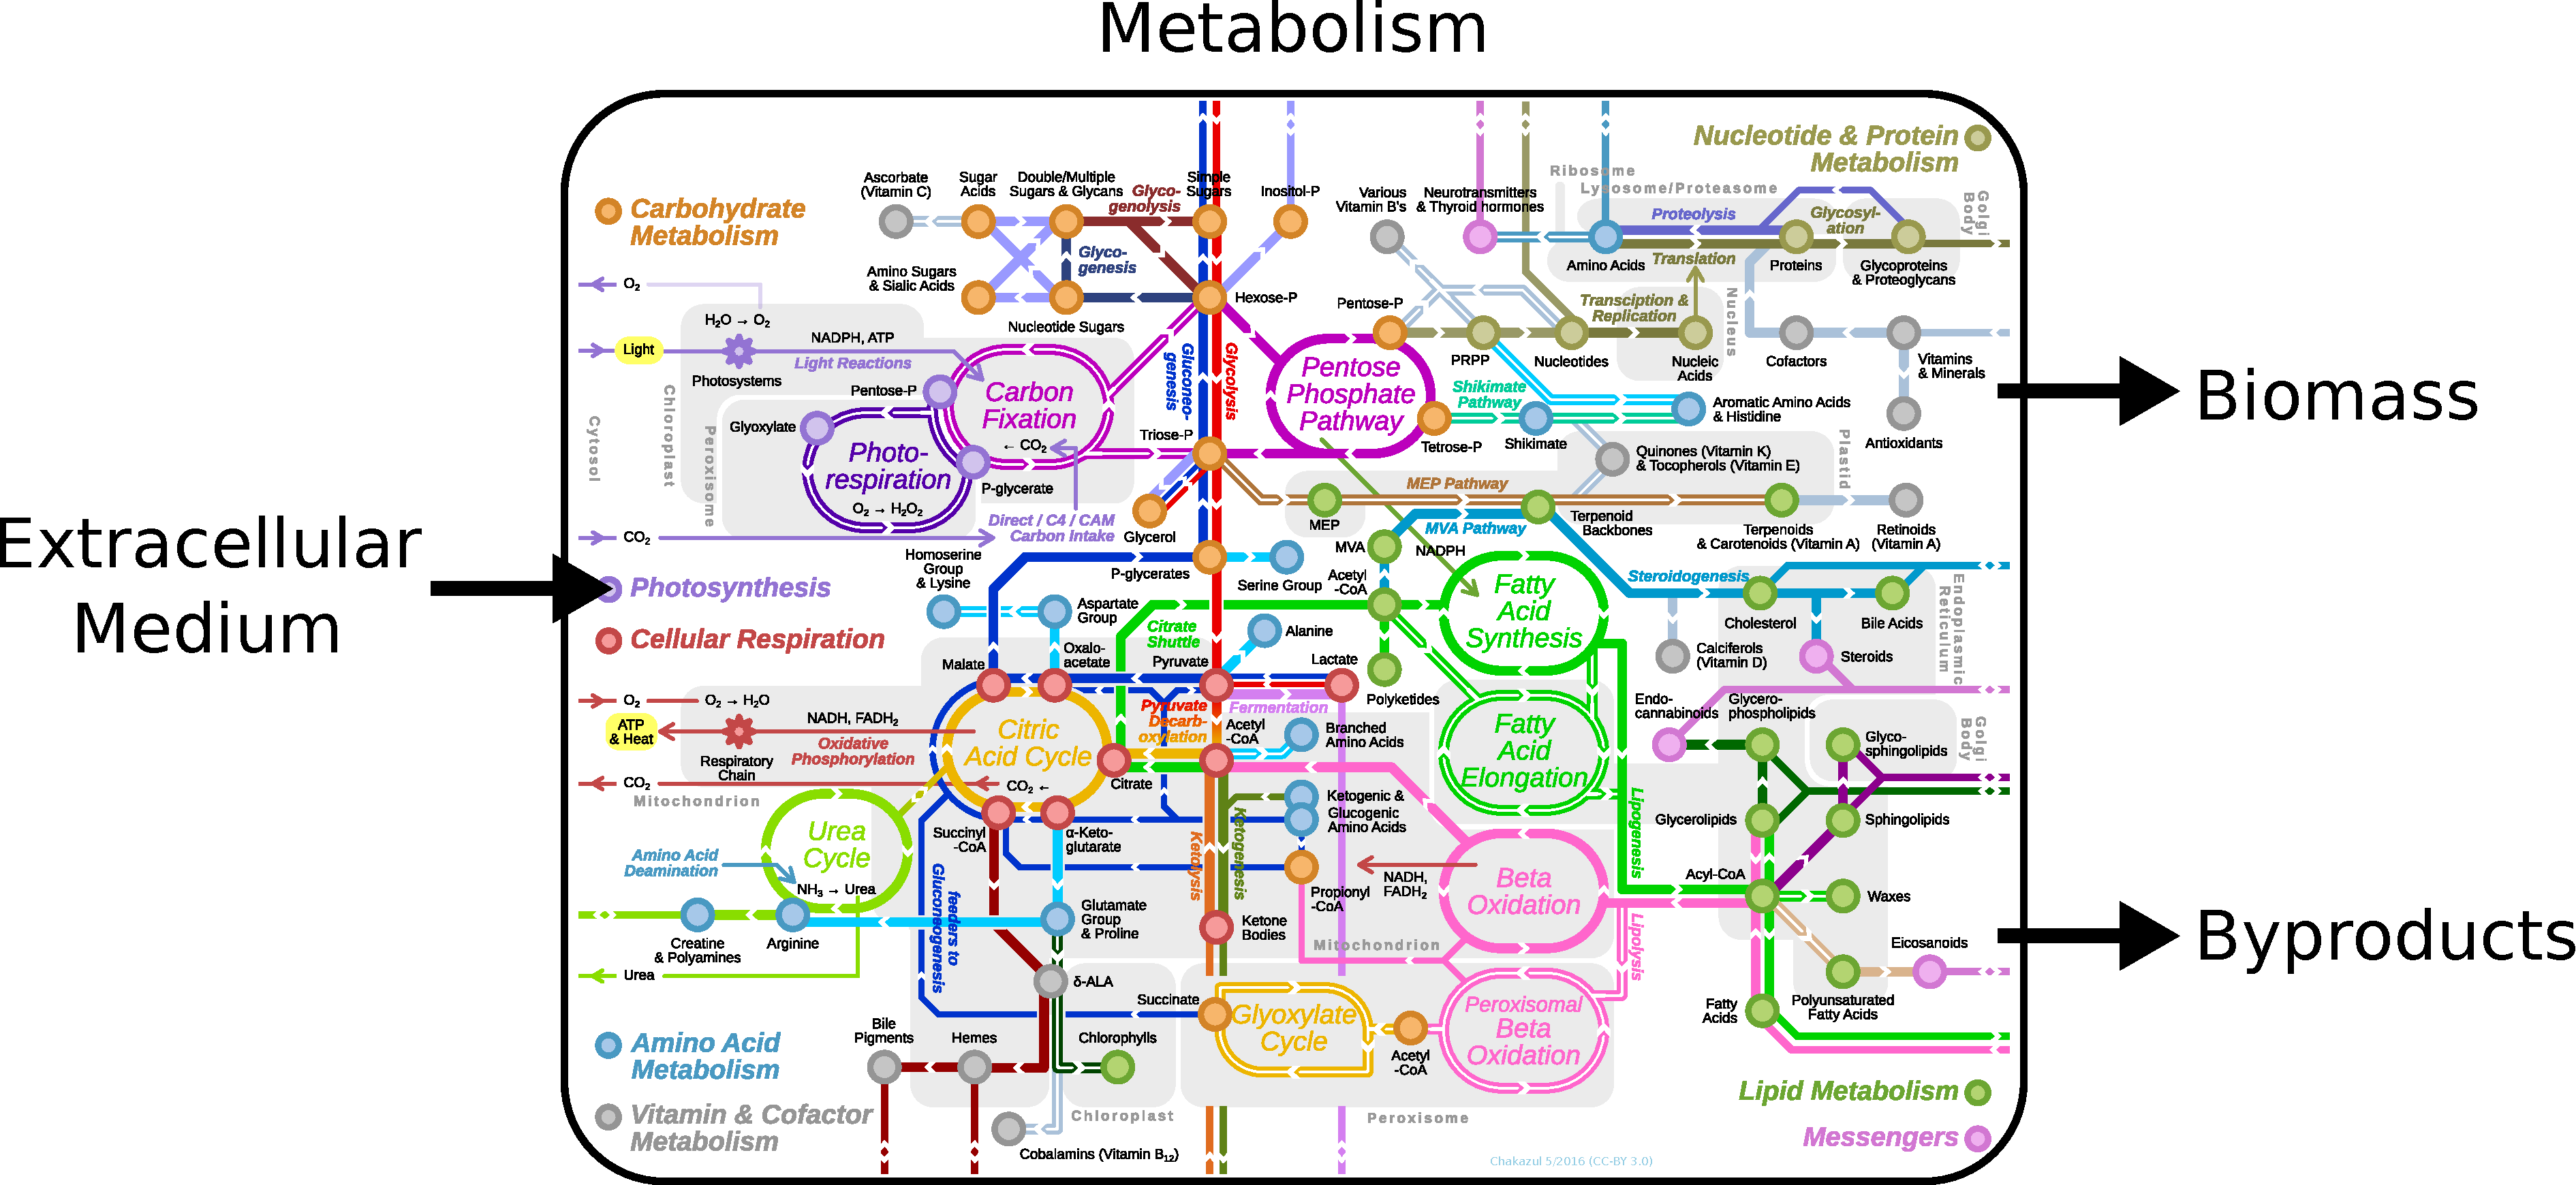
\includegraphics[width=\linewidth]{intro}
  \end{figure}
  3 central constraints:
  \begin{itemize}
    \item Conservation of mass.
    \item Catalytic capacities.
    \item Maximal compartment densities.
  \end{itemize}
\end{frame}

\begin{frame}{\textit{E. coli} SBML model}
  Illustration with compartments
  species
  reactions to genes mapping
\end{frame}

\begin{frame}{Enzyme synthesis reactions}
  From the SBML model we need to:
  \begin{enumerate}
    \item Map genes to protein information (amino acids, cofactors, stoichiometry).
    \item Add assembly costs of proteins (ATP/GTP used by translation, folding or translocation).
    \item Add machinery costs needed (ribosomes, chaperones, translocons).
    \item Deduce enzyme assembly costs.
  \end{enumerate}
\end{frame}

\begin{frame}{Other missing information}
  \begin{itemize}
    \item Enzyme efficiencies.
    \item Machinery efficiencies.
    \item Compartment density limitations.
  \end{itemize}
  All these parameters may be growth-rate dependent.
\end{frame}

\begin{frame}{RBAcell philosophy}
  \begin{itemize}
    \item Take a step back from SBML.
    \item XML format for interoperability (such as converting to SBML).
    \item Describe minimal information needed for RBA models.
    \item Uses cellular processes as a way to describe generic information.
  \end{itemize}
\end{frame}

\begin{frame}{RBA cell: overview of files}
  \begin{itemize}
    \item metabolism.xml: compartments, metabolites, metabolic reactions.
    \item parameters.xml: parameters and functions.
    \item proteins.xml, rnas.xml, dna.xml: polymer information.
    \item processes.xml: cellular processes.
    \item targets.xml: biomass targets.
    \item density.xml: maximal compartment densities.
    \item medium.tsv: external medium concentrations.
  \end{itemize}
\end{frame}

\begin{frame}{Polymers}
  \begin{figure}
    \centering
    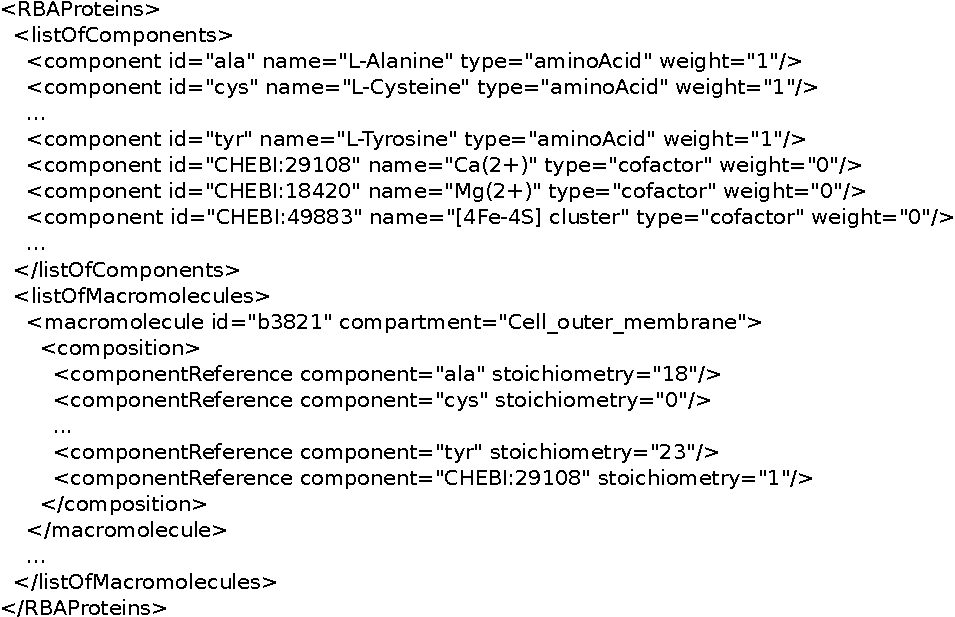
\includegraphics[width=\linewidth]{polymers}
  \end{figure}
  Components ids do NOT match SBML ids.
\end{frame}

\begin{frame}{Processing Maps}
  \begin{figure}
    \centering
    \includegraphics[width=\linewidth]{processing_map}
  \end{figure}
\end{frame}

\begin{frame}{Process}
  \begin{figure}
    \centering
    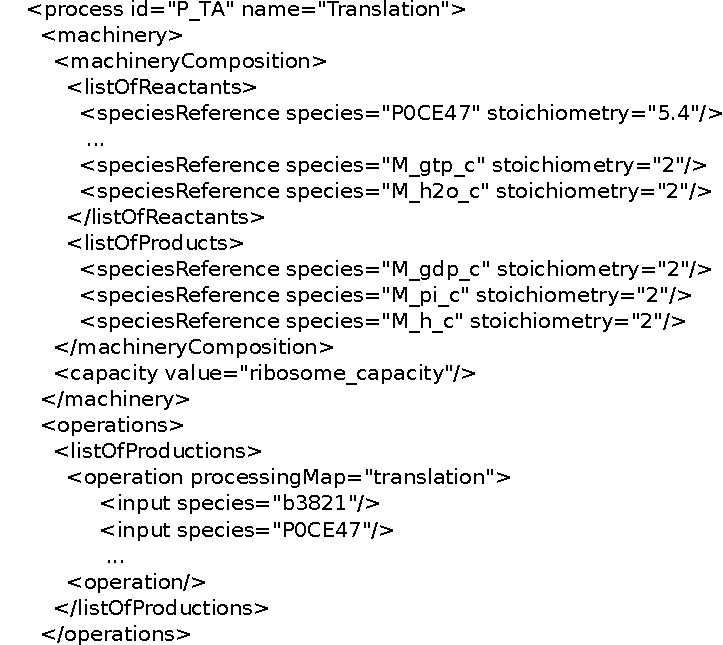
\includegraphics[width=\linewidth]{process}
  \end{figure}
\end{frame}

\begin{frame}{Combining processes}
  \begin{figure}
    \centering
    \includegraphics[width=\linewidth]{combining_processes}
  \end{figure}
\end{frame}

\begin{frame}{Polymer usage}
  \textbf{Biomass targets}
  \begin{figure}
    \centering
    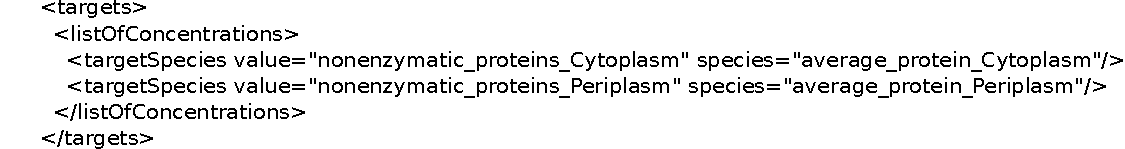
\includegraphics[width=\linewidth]{targets}
  \end{figure}
  \textbf{Enzymes}
  \begin{figure}
    \centering
    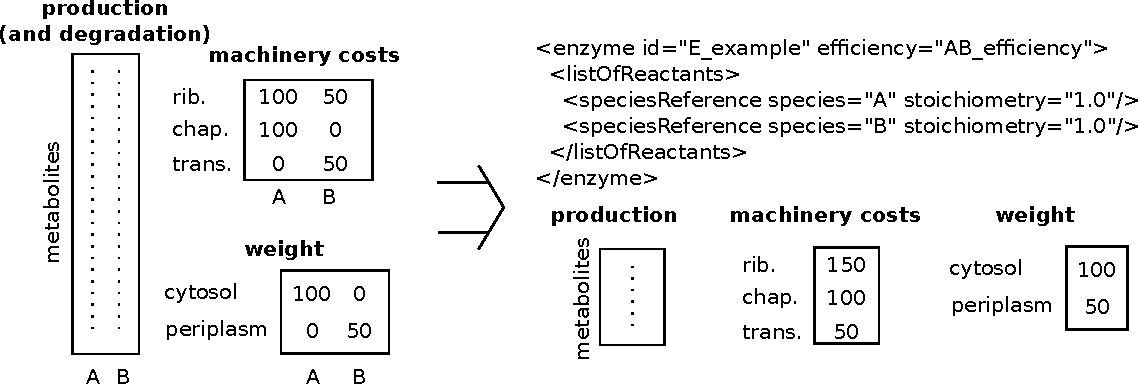
\includegraphics[width=\linewidth]{enzyme}
  \end{figure}
\end{frame}

\begin{frame}{Functions}
  In RBAcell, we use predefined function types and a variable attribute:
  \begin{figure}
    \centering
    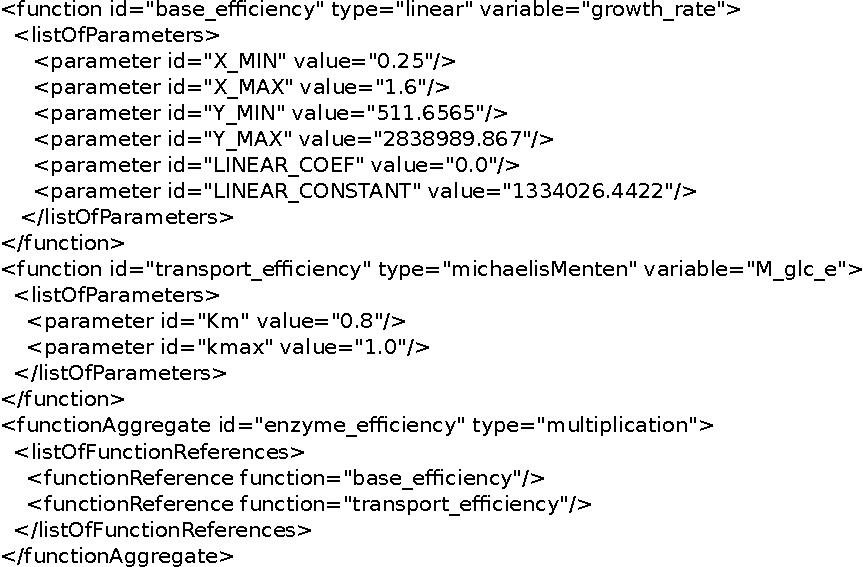
\includegraphics[width=\linewidth]{functions}
  \end{figure}
\end{frame}

\begin{frame}{Density constraints}
  Current implementation:
  \begin{figure}
    \centering
    \includegraphics[width=\linewidth]{density}
  \end{figure}
  More generic (future?) implementation:
  \begin{figure}
    \centering
    \includegraphics[width=\linewidth]{density_future}
  \end{figure}
\end{frame}

\begin{frame}{Format conversion and solving}
  \begin{figure}
    \centering
    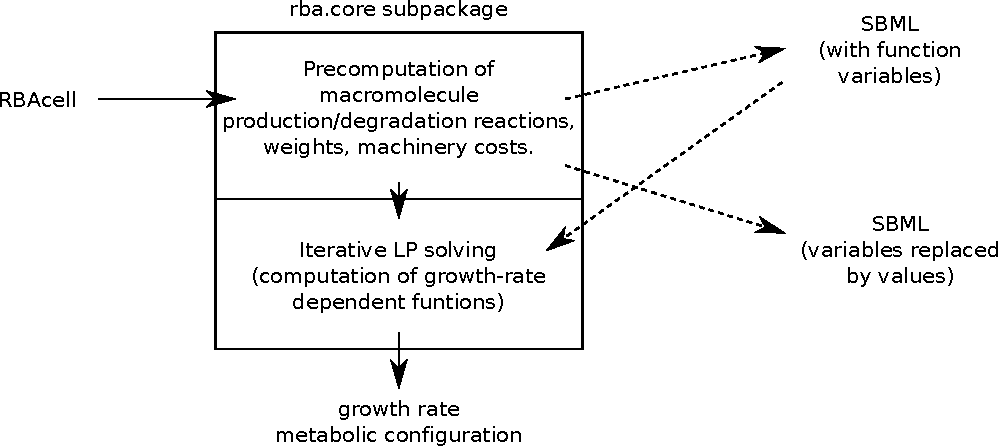
\includegraphics[width=\linewidth]{solving}
  \end{figure}
\end{frame}

\begin{frame}{Conclusions and perspectives}
  \begin{itemize}
    \item RBAcell is centered on cellular processes: flexible descriptions
    of polymer synthesis.
    \item Processes are mostly species-independent: we used the same set of processes to
    generate models for \textit{B. subtilis}, \textit{E. coli}, \textit{R. solanacearum}
    (only processing maps needed to be adapted).
    \item Next step: create a converter towards an SBML format
    (enzymes using RAM format?, functions?, density constraints?).
  \end{itemize}
\end{frame}

% ==========
%  Appendix
% ==========
\appendix
\newcounter{finalframe}
\setcounter{finalframe}{\value{framenumber}}

% % % % % % % % % % % ADD APPENDIX FRAMES HERE % % % % % % % % % % % % %

\setcounter{framenumber}{\value{finalframe}}

\end{document}
